\documentclass[10pt]{article}
\usepackage[margin=.78in]{geometry}
\usepackage{amsmath,amssymb,amsthm,booktabs,microtype,enumitem,hyperref,float,array,tabularx}
\usepackage[T1]{fontenc}
\usepackage{lmodern}
\usepackage{tikz}
\usetikzlibrary{arrows.meta,positioning,fit,calc,shapes.geometric}
\setlist{nosep,leftmargin=*}
\hypersetup{colorlinks=true,linkcolor=blue,urlcolor=blue,hypertexnames=false}
\newtheorem{definition}{Definition}
\newtheorem{principle}{Reporting principle}
\newcolumntype{Y}{>{\raggedright\arraybackslash}X}

\title{Distributed Learned Computation:\\Humans, LLMs, Tools, and Services as Heterogeneous Computational Networks}
\author{Paper 0.2 --- Position and Formal Inception}
\date{August 2026}

\begin{document}
\maketitle

\begin{abstract}
What changes when the relevant computational unit is not one learned model, but a network of learned models, humans, tools, services, and persistent memory? We propose a typed, stateful graph formalism for this question. A node exposes an interface-level transition and a multidimensional descriptor of capability, cost, latency, reliability, adaptability, memory, and iteration characteristics. Edges specify admissible message transformations; a router constructs a stateful execution under finite budgets. This abstraction permits system-level accounting without asserting that humans, language models, databases, and interpreters are internally or cognitively equivalent. It also separates five claims often collapsed in discussions of agents: component competence, route availability, route acquisition, execution reliability, and resource-bounded system closure. We develop reliability and verification accounting, locate task-defining computation in representative workflows, and connect the framework to distributed cognition, cognitive artifacts, distributed systems, multi-agent systems, human--AI collaboration, and tool-using language models. This is an inception and measurement framework, not evidence that distribution guarantees greater intelligence, mathematical closure, or any conclusion about consciousness.
\end{abstract}

\section{From learned machines to heterogeneous networks}

Paper 0.1 asks what Transformer-centered machines can represent, acquire, compose, and execute under explicit resources. A deployed computational process is often wider. A scientist supplies goals and judgments; an LLM proposes code; an interpreter executes it; a simulator produces observations; a database preserves state; tests reject some failures; and a human decides whether to continue. No single component realizes the complete workflow.

The natural unit of analysis is therefore sometimes a heterogeneous computational network. The proposal is operational: record which state transformations occur, which interfaces make them reachable, where task-defining work is performed, and what finite resources and failure modes govern the route. It is not the metaphysical claim that every participating artifact is literally part of a mind.

Three cautions organize the paper. First, a common node notation is an interface abstraction, not an assertion of internal equivalence. Second, adding nodes can add latency, ambiguity, correlated failure, or inaccessible capability; it need not improve the system. Third, a finite network run can support only a resource-bounded system signature, not mathematical closure.

\section{Typed stateful computational graphs}

\subsection{Nodes, interfaces, and state}

\begin{definition}[Heterogeneous computational graph]
A heterogeneous computational graph is
\[
\mathcal G=(V,E,\Sigma,\mathcal R),
\]
where each vertex $v_i\in V$ exposes a partial, typed, stateful transition
\[
N_i:X_i\times S_i\rightharpoonup Y_i\times S_i',
\]
$\Sigma$ is shared workflow state, $E$ contains typed interfaces, and $\mathcal R$ is a routing policy or protocol. An edge $e_{ij}$ carries a partial adapter
\[
\phi_{ij}:Y_i\times\Sigma\rightharpoonup X_j\times\Sigma
\]
that validates, serializes, authorizes, and transports a result. Undefined transitions include schema rejection, unavailable services, forbidden actions, and unsupported inputs.
\end{definition}

The explicit adapter matters. Text returned by an LLM is not automatically executable code; a database row is not automatically a model prompt; and a human instruction may be ambiguous. Schemas, parsers, permissions, prompts, and physical displays are computational interfaces with their own loss and failure modes.

At time $t$, a global configuration can be written
\[
z_t=(g,\Sigma_t,s_{1,t},\ldots,s_{n,t},h_t,b_t),
\]
where $g$ is the goal, $h_t$ is the message/event history, and $b_t$ is the remaining budget. The router selects a node, adapter, arguments, and control action:
\[
\mathcal R(z_t)=(i_t,e_t,x_t,\textsc{continue/stop/escalate}).
\]
The router may be programmed, learned, human, or itself distributed. Treating it as free would hide the central acquisition and coordination problem.

\subsection{Node descriptors are vectors, not scores}

For each node retain the descriptor requested by the network analysis,
\[
\chi_i=(\mathcal F_i,c_i,\ell_i,r_i,a_i,m_i,\kappa_i).
\]
Here $\mathcal F_i$ is a supported capability family; $c_i$ cost; $\ell_i$ latency; $r_i$ reliability; $a_i$ adaptability or generalization; $m_i$ accessible state capacity; and $\kappa_i$ iteration or closure characteristics. In careful use these are not constants: they are indexed by task distribution $D$, interface schema $q$, and budget $B$, for example $r_i(D,q,B)$.

\begin{table}[H]
\centering\small
\setlength{\tabcolsep}{5pt}
\begin{tabularx}{\linewidth}{>{\raggedright\arraybackslash}p{.13\linewidth}YYYYY}
\toprule
Node type & Typical strength & Typical state & Characteristic failure & Adaptation & Timing\\
\midrule
Human & grounded judgment, reframing & working and external memory & fatigue, bias, inconsistency & broad, experience-dependent & slow/variable\\
LLM & semantic transformation, flexible interface & context and external scratchpad & distribution shift, fabrication, control error & learned; prompt/context sensitive & fast/probabilistic\\
Database & indexed persistent records & large durable store & stale data, schema/query error & narrow updates & predictable\\
Calculator/CAS & exact declared transforms & small typed expression state & invalid input, unsupported operation & narrow & fast\\
Interpreter & programmable execution & program, heap, files & program defect, timeout, unsafe action & depends on supplied program & workload-dependent\\
Verifier & rejection/checking on a language & specification and evidence & false acceptance or incomplete coverage & usually narrow & additional cost\\
\bottomrule
\end{tabularx}
\caption{Interface-level contrasts. Entries are tendencies under declared tasks, not intrinsic rankings or claims of cognitive equivalence.}
\label{tab:nodes}
\end{table}

\subsection{A network view}

\begin{figure}[H]
\centering
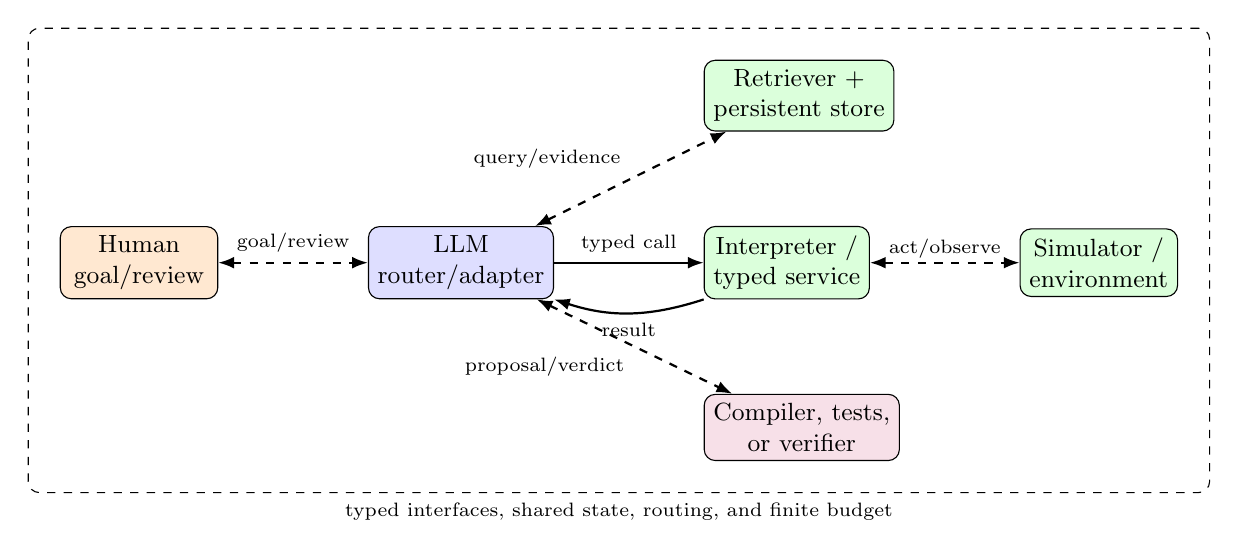
\begin{tikzpicture}[
  node distance=12mm and 19mm,
  box/.style={draw,rounded corners,align=center,minimum height=8mm,minimum width=20mm,font=\small},
  human/.style={box,fill=orange!18}, learned/.style={box,fill=blue!13},
  service/.style={box,fill=green!14}, verify/.style={box,fill=purple!12},
  edge/.style={-{Latex[length=2mm]},thick}, feedback/.style={{Latex[length=2mm]}-{Latex[length=2mm]},thick,dashed}
]
\node[human] (human) {Human\\goal/review};
\node[learned,right=of human] (llm) {LLM\\router/adapter};
\node[service,above right=of llm] (store) {Retriever +\\persistent store};
\node[service,right=of llm] (exec) {Interpreter /\\typed service};
\node[verify,below right=of llm] (check) {Compiler, tests,\\or verifier};
\node[service,right=of exec] (world) {Simulator /\\environment};
\draw[feedback] (human) -- node[above,font=\scriptsize]{goal/review} (llm);
\draw[feedback] (llm) -- node[above left,font=\scriptsize]{query/evidence} (store);
\draw[edge] (llm) -- node[above,font=\scriptsize]{typed call} (exec);
\draw[edge,bend left=18] (exec.south west) to node[below,font=\scriptsize]{result} (llm.south east);
\draw[feedback] (llm) -- node[below left,font=\scriptsize]{proposal/verdict} (check);
\draw[feedback] (exec) -- node[midway,above,fill=white,inner sep=1pt,font=\scriptsize]{act/observe} (world);
\node[draw,dashed,rounded corners,fit=(human)(store)(world)(check),inner sep=4mm,label={[font=\scriptsize]below:typed interfaces, shared state, routing, and finite budget}] {};
\end{tikzpicture}
\caption{One heterogeneous topology. Arrow labels denote typed interfaces, not transparent access. Routing, validation, state update, and stopping are part of the computation.}
\label{fig:network}
\end{figure}

\section{Routes and the location of computation}

For goal $g$, an execution trace is more than a node list:
\[
\pi_g=((z_0,i_0,e_0,x_0,y_0),\ldots,(z_T,i_T,e_T,x_T,y_T)).
\]
The shorthand $(N_{i_1},\ldots,N_{i_T})$ is useful for a diagram, but ordinary composition $N_{i_T}\circ\cdots\circ N_{i_1}$ is generally ill-typed and misses branching, retries, shared-state mutation, and human intervention.

An orchestrator may need to decompose a goal, select a node, form valid arguments, interpret the result, verify it, update state, and stop. Corresponding conditional measurements include
\[
P_{\rm decompose},\ P_{\rm select},\ P_{\rm parameterize},\ P_{\rm integrate},\\
P_{\rm verify},\ P_{\rm continue},\ P_{\rm stop}.
\]
These are empirical capabilities, not a definition of intelligence. A perfect solver behind an unusable interface is unreachable; a perfect call to a closure oracle does not show that the controller learned closure.

\begin{principle}[Computation-location record]
Every system result should name the component that performs the benchmark-defining transformation. Distinguish local execution, controller-side composition, delegated search/closure, generated-program execution, verification, and human judgment.
\end{principle}

For example, repeated calls to \texttt{parent(x)} leave state update and termination with the route. A single \texttt{root(x)} call delegates the traversal. Generating a loop and sending it to an interpreter moves iteration into the runtime while leaving program synthesis, serialization, result integration, and perhaps verification with other nodes. Equivalent computability does not imply equivalent acquisition probability, reliability, latency, or description cost.

\section{Reachability and resource-bounded system closure}

Let $\mathcal F_i(D,B)$ denote the functions node $i$ can execute to a declared gate on distribution $D$ under budget $B$. Define the reachable family
\[
\mathcal F_{\mathcal G}^{\rm reach}(D,B,\mathcal R)
\]
as functions executed by legal routed traces whose total calls, tokens, time, memory, permissions, and cost fit $B$. In general,
\[
\mathcal F_{\mathcal G}^{\rm reach}(D,B,\mathcal R)
\ \text{need not equal}\ \bigcup_i\mathcal F_i(D,B),
\]
and
\[
\mathcal F_{\mathcal G}^{\rm reach}(D,B,\mathcal R)
\subseteq
\left\langle\mathcal F_1,\ldots,\mathcal F_n\right\rangle_{E,\Sigma,\mathcal R,B}.
\]
Equality can hold in a degenerate graph. Routed composition can realize a transformation absent from every isolated node, while inaccessible interfaces or bad routing can prevent the network from using a nominally available node function.

Suppose a task family has complexity $K$, such as the number of local transitions. Node $i$ may have a measured contiguous frontier $K_i$. A routed network may have $K_{\mathcal G}>K_i$ because it externalizes memory, delegates transitions, or executes a generated program. This motivates a finite object rather than a universal closure claim.

\begin{definition}[System-level closure signature]
For a fixed network, routing protocol, evaluation distribution, and resource budget, define
\[
\Sigma_{\mathcal G,B}=(K_{\rm train},\mathcal K_{\rm test},K_{\rm prefix},
\rho_{\rm route},\rho_{\rm step},\rho_{\rm stop},g(K),f_{\rm fail},C(K)),
\]
where $K_{\rm prefix}$ is the largest contiguous tested prefix passing a multi-run gate, $\rho$ records routing, transition, and stopping reliability, $g(K)$ is observed trace-length scaling, $f_{\rm fail}$ is the first classified failure, and $C(K)$ is measured resource cost. This signature is finite empirical evidence, not the assertion $\forall K<\infty$.
\end{definition}

An LLM that fails to compute $f^{1000}$ internally may write a loop that an interpreter executes. If the routed system passes, the system frontier has increased under the tested budget. The LLM contribution may be program synthesis and integration; the interpreter supplies iteration and memory. The conclusion remains bounded by context, calls, runtime, memory, language semantics, and evaluation coverage.

\section{Reliability, verification, and redundancy}

For a realized path, the exact chain rule is
\[
P(\text{all required events})=\prod_{t=1}^{T}
P(E_t\mid E_1,\ldots,E_{t-1}).
\]
The simpler $\prod_t r_t$ is valid only as an independent, stationary baseline. Heterogeneous workflows commonly violate it: one malformed assumption can corrupt several downstream nodes; retries share the same prompt; tests correlate with the implementation; and human reviewers can miss the same ambiguity as the model.

A verification topology routes an output through a checker before accepting or acting on it. Examples include compiler and test feedback for code, proof checking for formal derivations, schema validation for API calls, a calculator for arithmetic, replication for simulations, and human escalation for underspecified or high-impact decisions. Verification is not free and not synonymous with correctness. Report its domain, false-acceptance and false-rejection behavior, coverage of the target failure modes, independence from the producer, added latency/cost, retry policy, and escalation rule.

\begin{table}[H]
\centering\small
\begin{tabularx}{\linewidth}{>{\raggedright\arraybackslash}p{.18\linewidth}YYYY}
\toprule
Mechanism & Potential benefit & Added resource & Characteristic limitation & Required measurement\\
\midrule
Retry & recovers transient failure & calls/time & repeats systematic error & conditional success by attempt\\
Redundancy & alternative proposal/path & nodes/cost & correlated models or sources & error correlation, aggregation rule\\
Deterministic check & rejects typed violations & verifier/time & incomplete specification & acceptance coverage\\
Human escalation & contextual judgment & attention/latency & fatigue and ambiguity & trigger, agreement, turnaround\\
Persistent log & audit and recovery & storage/privacy & stale or sensitive state & provenance, retention, consistency\\
\bottomrule
\end{tabularx}
\caption{Verification changes topology and budget. Its benefit is an empirical question conditional on checker coverage.}
\label{tab:verification}
\end{table}

\section{Representative workflows}

\begin{table}[H]
\centering\scriptsize
\begin{tabularx}{\linewidth}{>{\raggedright\arraybackslash}p{.14\linewidth}>{\raggedright\arraybackslash}p{.31\linewidth}YYY}
\toprule
Workflow & Representative route & Distributed contribution & Task-defining location & Principal boundary\\
\midrule
Scientific & human $\to$ LLM $\to$ Python $\to$ simulator $\to$ LLM $\to$ human & hypothesis, program, execution, interpretation & split across model, runtime, simulator, judgment & model/data validity, replication\\
Coding & human $\to$ coding model $\to$ compiler/tests $\to$ repository $\to$ model & proposal, deterministic feedback, persistent state & generated patch plus toolchain & test coverage, stopping, unsafe change\\
Enterprise & human $\leftrightarrow$ LLM $\leftrightarrow$ APIs/SQL/rules & semantic routing among typed services & often service or business-rule engine & authorization, schema, policy\\
Research & LLM $\leftrightarrow$ retriever/GraphRAG/database $\to$ human review & evidence access, synthesis, review & retrieval/search semantics plus integration & source sufficiency, provenance\\
Calculator/CAS & human/LLM $\to$ symbolic engine $\to$ human/LLM & dispatch plus exact transform & external engine & serialization, unsupported operations\\
\bottomrule
\end{tabularx}
\caption{Workflows illustrate distributed computation, not internal equivalence among their nodes.}
\label{tab:workflows}
\end{table}

RAG changes available information; iterative RAG additionally changes routing. GraphRAG can expose a local-neighbor primitive, a substantial aggregation, or a complete path/search service, so the product name alone does not determine computational semantics. ReAct interleaves reasoning traces, actions, and observations; MRKL routes among modules; Toolformer studies acquisition of calls; PAL delegates execution of generated programs \cite{lewis2020,edge2024,yao2023,karpas2022,schick2023,gao2023}. Each should be described by its actual node interfaces and by where the benchmark-defining operation occurs.

\section{Relation to neighboring traditions}

\subsection{Distributed cognition and cognitive artifacts}

Distributed cognition studies cognitive activity across people, representations, artifacts, and environments rather than locating every explanatory state inside one individual \cite{hutchins1995}. Work on cognitive artifacts similarly emphasizes that representational tools can transform the tasks users perform \cite{norman1991}. This motivates system-level analysis of state and interfaces.

The extended-mind thesis is stronger: Clark and Chalmers ask when environmental elements may constitute parts of a cognitive process \cite{clark1998}. Our graph formalism does not decide that metaphysical question. Participation in an operational computation is sufficient for the accounting developed here; it does not entail mentality, consciousness, agency, or moral status.

\subsection{Distributed systems, collective intelligence, and multi-agent systems}

Distributed systems contribute precise concerns about message passing, scheduling, partial failure, retries, consistency, authorization, and resource allocation \cite{tanenbaum2017}. Learned nodes add distribution-sensitive semantics and interfaces that may be underspecified. Collective-intelligence research asks how group structures aggregate information and action; the present formalism contributes typed computational routes and resource/failure accounting rather than a scalar group-intelligence measure \cite{malone2015}.

Multi-agent systems study interacting autonomous agents, coordination, and distributed problem solving \cite{wooldridge2009}. A multi-LLM system is a homogeneous special case only at a coarse node-type level. Copies of one model may share training-induced errors, and adding agents does not itself enlarge the reachable family. Topology, role differentiation, state, communication, aggregation, and budget determine the change.

\subsection{Human--AI and socio-technical systems}

Human-in-the-loop systems place people in labeling, control, review, exception handling, or governance roles. HCI emphasizes interaction design and the gap between nominal functionality and usable capability; socio-technical analysis emphasizes that organizational rules, incentives, authority, and work practice shape system behavior. The graph should therefore include authorization and escalation interfaces rather than idealize the human as a cost-free oracle. Empirical reports should measure workload, delay, disagreement, override, and which errors reach the human.

\section{Implications for comparisons with human intelligence}

A model-only benchmark and a human-with-artifacts benchmark compare different machines. Humans ordinarily use language, notation, collaborators, search, calculators, computers, and durable memory. LLM-centered applications likewise use retrieval, interpreters, databases, and verification. Fair comparison requires declaring the allowed network and budget on both sides.

This does not reduce intelligence to routing. Goal formation, grounding, learning, adaptation, representation, social understanding, and judgment may be decisive node capabilities. Nor does system success license the statement that an orchestrating LLM internally possesses every delegated competence. A useful report separates:
\begin{enumerate}
  \item component capability and acquisition;
  \item interface accessibility and information sufficiency;
  \item route selection and state maintenance;
  \item execution and termination reliability;
  \item verification coverage and recovery;
  \item total resource cost and where the defining computation occurs.
\end{enumerate}

\section{Research program}

The inception yields testable questions. When does a heterogeneous route realize a function unavailable to every isolated node under matched budgets? When is a gain instead better acquisition or reliability for a computation already representable? Which interface schemas enable compositional reuse? How do routing errors correlate with tool errors? When do deterministic checks improve end-to-end reliability, and when do specification gaps create false confidence? How does persistent state change train-short/test-long behavior? Which human escalation policies improve accuracy without unacceptable workload? Can a measured system-level closure signature survive new task distributions, longer traces, tighter budgets, and adversarial interface failures?

A minimal experimental record should contain a graph/schema version, node descriptors, task distribution, routing policy, message traces, state mutations, budgets, per-interface outcomes, computation-location labels, verifier decisions, retries, stopping, and cross-run gates. Ablations should remove or weaken one interface at a time. Controller-matched local tools should precede closure or interpreter services, because the latter may delegate the task being attributed to the learned route.

\section{Conclusion}

Heterogeneous networks are a useful computational abstraction when meaningful work is distributed among humans, learned models, deterministic services, tools, and persistent representations. The abstraction earns its keep only when interfaces, state, routing, budgets, and failure are explicit. It then becomes possible to say precisely whether a system gained reachable computation, route acquisition, execution reliability, verification, or efficiency---and where the work occurred. It does not imply that nodes are internally equivalent, that distribution guarantees intelligence, that finite success establishes closure, or that an operational network settles questions about mind or consciousness.

\begin{sloppypar}
\begin{thebibliography}{99}
\raggedright
\bibitem{hutchins1995} E. Hutchins. \emph{Cognition in the Wild}. MIT Press, 1995. doi:10.7551/mitpress/1881.001.0001.
\bibitem{clark1998} A. Clark and D. Chalmers. The Extended Mind. \emph{Analysis}, 58(1):7--19, 1998. doi:10.1093/analys/58.1.7.
\bibitem{norman1991} D. A. Norman. Cognitive Artifacts. In J. M. Carroll, ed., \emph{Designing Interaction: Psychology at the Human--Computer Interface}. Cambridge University Press, 1991.
\bibitem{malone2015} T. W. Malone and M. S. Bernstein, eds. \emph{Handbook of Collective Intelligence}. MIT Press, 2015.
\bibitem{tanenbaum2017} A. S. Tanenbaum and M. van Steen. \emph{Distributed Systems: Principles and Paradigms}, 3rd ed. distributed-systems.net, 2017.
\bibitem{wooldridge2009} M. Wooldridge. \emph{An Introduction to MultiAgent Systems}, 2nd ed. Wiley, 2009.
\bibitem{lewis2020} P. Lewis et al. Retrieval-Augmented Generation for Knowledge-Intensive NLP Tasks. \emph{NeurIPS}, 2020.
\bibitem{karpas2022} E. Karpas et al. MRKL Systems: A Modular, Neuro-Symbolic Architecture That Combines Large Language Models, External Knowledge Sources and Discrete Reasoning. arXiv:2205.00445, 2022.
\bibitem{schick2023} T. Schick et al. Toolformer: Language Models Can Teach Themselves to Use Tools. \emph{NeurIPS}, 2023.
\bibitem{gao2023} L. Gao et al. PAL: Program-Aided Language Models. \emph{ICML}, 2023.
\bibitem{yao2023} S. Yao et al. ReAct: Synergizing Reasoning and Acting in Language Models. \emph{ICLR}, 2023.
\bibitem{edge2024} D. Edge et al. From Local to Global: A Graph RAG Approach to Query-Focused Summarization. arXiv:2404.16130, 2024.
\end{thebibliography}
\end{sloppypar}

\end{document}
